\chapter{Flujo de trabajo para la implementación de software para GNC embebido}
\label{ch:especifico2}

Como se pudo observar en el capítulo \ref{ch:especifico1}, se realizó la selección de la tarjeta de desarrollo Zedboard para el desarrollo del proyecto, además de esto uno de los parámetros que se tomó en cuenta fue la compatibilidad de esta tarjeta con el flujo de trabajo de Yocto Project, es por esto que en este capítulo se pretenden establecer los flujos de trabajo para el prototipado de algoritmos de control de orientación y navegación para aplicaciones espaciales. Esto mediante el uso de MATLAB Simulink para tomar un caso de estudio como ejemplo, seguido de esto convertir el código por medio de la transformación de modelo de Simulink a un modelo de código C, esto con el objetivo de poder embeber el código C en una imagen mínima por medio del flujo de trabajo de Yocto Project y finalmente probar el mismo en la tarjeta de desarrollo seleccionada en el capítulo \ref{ch:especifico1} y de esta forma poder comparar los resultados obtenidos y el tiempo de ejecución que llevo la tarea en el computador y en el sistema embebido.


\begin{figure}[h!]
    \centering
    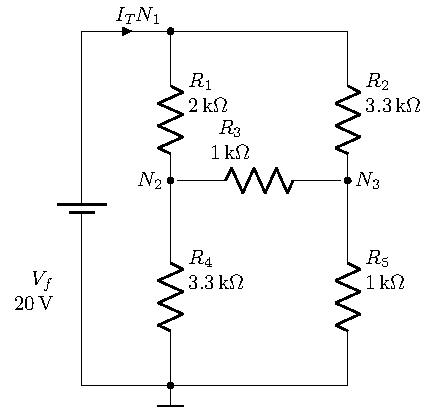
\includegraphics[width=0.3\textwidth]{fig/figtemplate.pdf}
    \caption{Diagrama general del flujo de trabajo propuesto}
    \label{fig:diagrama_flujo_trabajo}
\end{figure}


En la Figura \ref{fig:diagrama_flujo_trabajo}, se muestra un diagrama del flujo de trabajo general. En este capítulo se trabajará en la sección remarcada en rojo la cual engloba la generación del modelo utilizado como caso de estudio, la validación del mismo en MATLAB Simulink, la generación de un código en lenguaje C y la incorporación del mismo en el flujo de trabajo de Yocto Project.

\section{Flujo de trabajo de la aplicación Model 2 Model Transformation}

Para poder embeber el sistema se debe de hacer uso del MATLAB Simulink Coder, el cual tiene la capacidad de convertir un sistema de conrtol generado en MATLAB Simulink, en un codigo C, algunos de los parametros que se pueden configurar en este convertidor de modelos son:

\begin{itemize}
    \item 
\end{itemize}

A lo largo de este capitulo se definiran los parametros que se deben de utilar y el funcionamiento de estos dentro de la generacion del codigo C.

\section{Selección del caso de estudio}

Como caso de estudio se selecciono una aplicacion la cual permitiera una comparacion de resultados antes del procesado y despues del mismo, es por esto que se decidio implementar un filtro  de tipo xxx haciendo uso de los siguientes bloques de MATLAB Simulink. 

\begin{itemize}
    \item Onda seno
    \item Suma
    \item Función de transferencia
    \item Generador de archivo de salida
\end{itemize}

La configuracion seleccionada para el primer generador de onda seno es:

\begin{itemize}
    \item Amplitud = 1
    \item Bias = 0 
    \item Frecuencia = 1 rad/s
    \item Fase = 0 
    \item Tiempo de muestreo = 0 
\end{itemize}

Mientars que para la segunda onda se tiene la configuracion:

\begin{itemize}
    \item Amplitud = 1
    \item Bias = 0 
    \item Frecuencia = 12 rad/s
    \item Fase = 0 
    \item Tiempo de muestreo = 0 
\end{itemize}

Esto con el objetivo de sumar las ondas y que las mismas (explicar que pasa al sumar dos ondas de distinta frecuencia)

Por otro lado la funcion de transferencia a utilizar sera:

ingresar la funcion de transferencia

esto con el fin de separar las frecuencias anteriormente sumadas y obtener una salida con la (describir que se espera a la salida)

Estos bloques mencionados anteriormente se lococan como se muestra en la Figura \ref{}, de modo que se obtienen como salida del sistema 2 archivos, uno llamado xxx el cual contiene los datos crudos de la suma de las dos sennales y otro denomindado, xxxx el cual contiene los datos de la sennnal filtrada por la funcion de tranferencia. 

\subsection{Simulacion del caso de estudio en Matlab Simulink}\label{subsec:simulacion_caso_de_estudio}

Utilizando el diagrama de la Figura \ref{} asi como usando los parametros configurados anteriormente se colocan dos bloques de grafico en el diagrama como se muestra en la Figura \ref{}, esto con el objetivo de poder observar las senales de salida en cada uno de los puntos de interes. 

(imagen compuesta por dos graficos uno al lado del otro donde a la derecha mostremos las senales sumadas y a la derecha las senales filtradas)

Como se puede observar en la Figura \ref{} se puede observar la salida de la suma de las dos senales senoidales, por otro lado en la Figura \ref{} se puede observar la salida de la funcion de transferencia.

\subsubsection{Resultados obtenidos con la ejecución de la simulacionn}

Como se menciono anteriormente los resultados obtenidos se pueden observar en la Figura \ref{}, siendo la salida esperada de la funcion de transferencia ya que al ser un filtro paso xxx atenua las senales que sten por debajo de la frencuencia de corte que para este filtro es de xxx. Como la senal compuesta contiene una senal con frecuencia de xxxx y otra con frencuencia de xxxx es posible observar aun componentes de la frecuencia atenuada.

\subsection{Simulink coder}

Una vez comprobado el comportamiento esperado por el caso de estudio se puede proceder con la ejecucion del flujo de trabajo de MATLAB Simulink coder, esto con el fin de transformar el modelo generado en Simulink a un modelo de lenguaje de programacion C. Cabe destacar que para esta implementacion se utilizo el diagrama que se muestra en la Figura \ref{} ya que el mismo solamente contiene los archivos con los datos numericos del sistema y no contiene las salidas graficas agregadas en \ref{subsec:simulacion_caso_de_estudio}.


\subsection{Definicio de paramtetros}

Para la definicion de parametros, se debe de estar en el entorno de MATLAB Simulink, una vez en el entorno mencionado anteriormente se debe ir a la pestanna denominada Aplicaciones, como se muestra en la Figura \ref{}, se debera de seleccionar la aplicacion denominada Simulink Coder, cuando seleccionamos esta opcion se abrira una pestanna llamada Codigo C, como se pudo observar en la Figura \ref{}, una vez estemos en la pestanna de codigo C, debemos de ir a la opcion de configuracion de parametros, tal y como se muestra en la Figura \ref{}, una vez presionada la opcion se abre una ventana emergente como la que se muestra en la Figura \ref{}, en la pestanna denominada Solver se deberan de proporcionar los datos de Tiempo de inicio y Tiempo de finalzacion de la simulacion.

\subsubsection{seleccion del procesador objetivo}

Continuando en la seccion de configuracion de parametros ahora debemos de ir a la pestanna llamada Hardware Implementation, en donde deberemos de colocar los datos de Device Vendor el cual para nuestro caso seria ARM Compatible y el Device Type que seria un ARM Cortex-A de 32-bits tal y como se muestra en la Figura \ref{}.


\subsubsection{Seleccion del tipo de archivo de construccion}

Ahora bien, anteriormente configuramos los parametros de de tiempo de operacion y procesador de la tarjeta de desarrollo, ahora debemos de configurar el tipo de archivo que se utilizara para la generacion de los archivos, como se debera de realziar una compilacion cruzada se debe de elegit un tipo de archivo el cual nos permita compilar los binarios para la ejecucion del sistema sin importar el sistema operativo de la maquina host. Es por esto que se debe de seleccionar en la pestanna de Code Generation el Toolchain denominado CMake tal y como se muestra en la Figura \ref{}.


\subsubsection{Generacion de archivos de compilacion}

Una vez configurados todos los parametros mencionados anteriormente debemos de proceder con la construccion de los archivos, para esto se debe de ir a la barra de tareas a la opcion denominada como generar codigo, la misma se puede observar en la Figura \ref{}.

\subsection{Contenedor para compilacion de los binarios}

Para poder generar la compilacion cruzada es necesario crear un contenedor para poder utilizar Ubuntu 20.04 ya que esta version es la que presenta mayor compatibilidad con las dependencias contenidas en el flujo de trabajo de Yocto Porject que se utiliza. 

Para poder generar esta contenedor se hace uso del comando que se muestra en \ref{}, este comando se encarga de cnostruir la maquina dentro del entorno del contenedor. 

\subsubsection{Istalacion de programas en el contenedor}

Una vez generado el contenedor debemos de instalar en el mismo xxxxx y xxxxx las cuales son herramientas que nos ayudaran a compilar el programa generado en \ref{} para la arquitectura del procesador. 

\subsection{Compilacion de los binarios}

Para la compilacion de los binaros se debera hace uso del comando xxx por el cual se construira el makefile, una vez generado el make file se ejecuto el comando xxxx el cual da como salida los binarios requeridos para la ejecucion del programa. Los mismos se observan como se muestra en la Figura \ref{}. 

Una vez compilados los binarios se puede continuar con el flujo que se presneta en el diagrama que se muestra en la Figura XX, lo cual seria la implemetnacion de los binarios en una imagen de yocto.


\section{Flujo de Trabajo Herramienta desarrollada por mi persona}

Como se pudo observar anteriormente se realizo la compilacion cruzada de un caso de estudio, el mismo ahora se debe de implementar en un sistema operativo a la medida mediante el flujo de trabajo de Yocto Project, como se menciono en \ref{}, yocto project es un marco de trabajo utilizado para el desarrollo de sistemas embebidos especializado en la cosntruccion de distribuciones de linux a la medida. 

En el desarrollo de esta seccion se muestran los pasos que se siguieron para la generacion de la imagen minima, la integracion de una capa personalizada con el binario generado en \ref{} y la implementacion de la misma en la tarjeta de desarrollo seleccionada.

\subsection{Sistema operativo para desarrollo}

Como sistema operativo de desarrollo se utilizo Ubuntu 22.04 LTS, en una computadora con las siguientes caracteristicas 

\begin{itemize}
    \item Procesador - Intel Corei9-13980HX 
    \item Almecenamiento - 500 GB
    \item Memoria RAM - 16 GB 
\end{itemize}

\subsection{Generacion de un contenedor}

Para el desarrollo del marco de trabajo de Yocto se decidio implementar un contenedor, esto debido a que la version de yocto para la cual se encontraba un paquete de soporte para la tarjeta de desarrollo es Yocto Zeus 3.0, este fue liberado en el ano de xxxx por tanto no era soportado por la version de linux del computador de desarollo. 

\subsubsection{Creacion de un usuario no root}

Para el uso del marco de trabajo de Yocto se debe de generar un usuario no root, (explicar por que yocto no puede correr en un usuario root)

\subsection{Yocto Project}

Como se observo en \ref{}, yocto presenta flexibilidades a la hora de configurar un sistema permitiendo al desarrollador seleccionar paquetes especificos y personalizar el sistema operativo.

La version de yocto a utlizar se debe de clonar de \ref{}, segido de esto se debe de ir al branch de la version mencionada en \ref{} (Yocto Zeus). Ademas de clonar este repositorio se debe de ingresar al directorio denominado xxx y clonar dentro de el el repositorio \ref{} el cual contiene en su branch xxx la version de bsp requerida para generar una imagen para la tarjeta de desarrollo.


Algunas configuraciones adicionales que se deben de realizar se muestran e \ref{}.

\subsection{creacion de una capa de yocto}

Para la generacion de una capa de yocto de debe de utilzair el siguiente comando el cual se encargara de generar el arbol de directorios que se puede observar en la Figura \ref{}. Una vez implementado este comando se debe de hacer uso de este comando para poder agregar la capa al archivo denominado xxxx el cual contiene todas las rutas de acceso a las capas requeridas para generar la imagen.

\subsection{Caso de estudio}

\subsection{integracion del programa generado a la capa de Yocto}

Para la implementacion de la los binarios generados en \ref{}, se deben de generar algunos directarios, esto con el objetivo de mantener un entorno limpio y ordenado, para contener todos los directorios se genera un directorio llamado xxxx el cual dentro del mismo debera de contener un directorio llamado xxx el cual se encargara de contener el archivo de configuracion de la capa llamado xxxx el cual se genera mediante el comando que se observa en \ref{}, ademas de geenerar este archivo se debe de crear un directorio llamado xxxx que sera el encargado de contener los binarios compilados en \ref{}.

\subsubsection{.bb}

Como se menciono anteriormente el archivo llamado xxxx.bb es el encargado de la configuracion de la capa, el mismo contiene los comandos de instalacion y la direccion en donde se encontraran los binarios en el sistema de archivos de la imagen del sistema embebido.

La estructura que debe de contener ese archivo para instalar binarios en el sistema son las que se puden observar en \ref{}.

\subsection{Generacion de la imagen minima}

Antes de generar la imagen minima 

\subsection{Implementacion de la imagen minima en la tarjeta de desarrollo zedboard}
Como se debe de implementar el boot de la tarjeta, como se debe de implementar el  sistema de archivos
\subsection{Conexion de la tarjeta de desarrollo con el computador host}
diagrama de conexion y programas utilizados para llevar a cabo el enlace

\subsection{Ejecucion del caso de estudio y resultados}

\subsection{Comparacion de resultados}

\section{Reflexion final}